%%%%%%%%%%%%%%%%%%%%%%%%%%%%%%%%%%%%%%%%%%%%%%%%%%%%%%%%%%%%%%%%%%%%%%%%%%%%%%%%%%%%%%%%%%%%%%%%%%%%%%%%%%%%%%%%%%%%%%%%%%%%%%%%%%%%%%%%%%%%%%%%%%%%%%%%%%%%%%%%%%%
% Written By Michael Brodskiy
% Class: Fundamentals of Electronics
% Professor: M. Onabajo
%%%%%%%%%%%%%%%%%%%%%%%%%%%%%%%%%%%%%%%%%%%%%%%%%%%%%%%%%%%%%%%%%%%%%%%%%%%%%%%%%%%%%%%%%%%%%%%%%%%%%%%%%%%%%%%%%%%%%%%%%%%%%%%%%%%%%%%%%%%%%%%%%%%%%%%%%%%%%%%%%%%

\documentclass[12pt]{article} 
\usepackage{alphalph}
\usepackage[utf8]{inputenc}
\usepackage[russian,english]{babel}
\usepackage{titling}
\usepackage{amsmath}
\usepackage{graphicx}
\usepackage{enumitem}
\usepackage{amssymb}
\usepackage[super]{nth}
\usepackage{everysel}
\usepackage{ragged2e}
\usepackage{geometry}
\usepackage{multicol}
\usepackage{fancyhdr}
\usepackage{cancel}
\usepackage{siunitx}
\usepackage{physics}
\usepackage{tikz}
\usepackage{mathdots}
\usepackage{yhmath}
\usepackage{cancel}
\usepackage{color}
\usepackage{array}
\usepackage{multirow}
\usepackage{gensymb}
\usepackage{tabularx}
\usepackage{extarrows}
\usepackage{booktabs}
\usepackage{lastpage}
\usetikzlibrary{fadings}
\usetikzlibrary{patterns}
\usetikzlibrary{shadows.blur}
\usetikzlibrary{shapes}

\geometry{top=1.0in,bottom=1.0in,left=1.0in,right=1.0in}
\newcommand{\subtitle}[1]{%
  \posttitle{%
    \par\end{center}
    \begin{center}\large#1\end{center}
    \vskip0.5em}%

}
\usepackage{hyperref}
\hypersetup{
colorlinks=true,
linkcolor=blue,
filecolor=magenta,      
urlcolor=blue,
citecolor=blue,
}


\title{Homework 6}
\date{\today}
\author{Michael Brodskiy\\ \small Professor: M. Onabajo}

\begin{document}

\maketitle

\begin{enumerate}

  \item

    We may begin by finding the current flowing from the $-15[\si{\volt}]$ source. Since we know the voltage at the node above the resistor ($.7[\si{\volt}]$ due to $V_{BE}=.7[\si{\volt}]$ and being connected to ground), we may get:

    $$I_{-15}=\frac{15+.7}{150000}$$
    $$I_{-15}=104.67[\si{\micro\ampere}]$$

    We may write the equation for the voltage across both the $4.7[\si{\kilo\ohm}]$ and $47[\si{\kilo\ohm}]$ resistors as:

    $$V_{4.7k}=(I_{-15}+I_{B})(47k)$$
    $$V_{4.7k}=(I_{-15}+I_{B}+I_C)(4.7k)$$

    Putting these together, we find the KVL equation to be:

    $$15=(I_{-15}+I_B)(47k)+(I_{-15}+I_B+I_C)(4.7k)+.7$$

    Note that, per BJT equations, we know that:

    $$I_C=\beta I_B$$

    Using this, we combine the two equations to get:

    $$15=\left(11I_{-15}+\frac{(11+\beta)I_C}{\beta}\right)(4.7k)+.7$$

    Now, we substitute known values, and solve for $I_C$:

    $$14.3=[\left( 1.1514\cdot10^{-3} \right)+1.055I_C](4.7k)$$
    $$14.3=5.4116+4958.5I_C$$
    $$I_C=\frac{14.3-5.4116}{4958.5}$$
    $$\boxed{I_C=1.7926[\si{\milli\ampere}]}$$

    We can then obtain $V_{CE}$:

    $$V_{CE}=15-(4.7)\left( 1.7926+\frac{1.7926}{200}+104.67\cdot10^{-3} \right)$$
    $$\boxed{V_{CE}=6.04.07[\si{\volt}]}$$

  \item

    \begin{enumerate}

      \item 

        We may begin by writing the equation for the input of the circuit:

        $$V_{i}+R_BI_B-V_{BE}-9+8.2=0$$

        Substituting our known values, we obtain:

        $$V_{BE}-8000I_B=.2\sin(2000\pi t)-.8$$

        Using the load line characteristic plots in the provided figure, we may observe (approximately):

        $$\boxed{5\leq I_B\leq 50[\si{\micro\ampere}]}$$

        At the Q-point, we see:

        $$\boxed{I_{BQ}\approx 25[\si{\micro\ampere}]}$$

        At the output, we may find the equation as:

        $$V_{CE}-3000I_C=-9$$

        From this, we analyze the load-line plots to see:

        $$\boxed{-8.25\leq V_{CE}\leq -1.5[\si{\volt}]}$$

        Furthermore, we may see that, at the Q-point:

        $$\boxed{V_{CEQ}=-5.25[\si{\volt}]}$$

        Given that $V_o=V_{CE}+9$, we get:

        $$\boxed{V_o(t)=\left\{\begin{array}{ll} \text{min}, & .75\\\text{Q}, & 3.75\\ \text{max}, & 7.5\end{array}[\si{\volt}]}$$

          We may see that, because both the input and output are positive, this $pnp$ common-emitter amplifier \underline{does not invert} the signal.

      \item 

        \begin{enumerate}

          \item The circuit is constructed below:

            \begin{figure}[H]
              \centering
              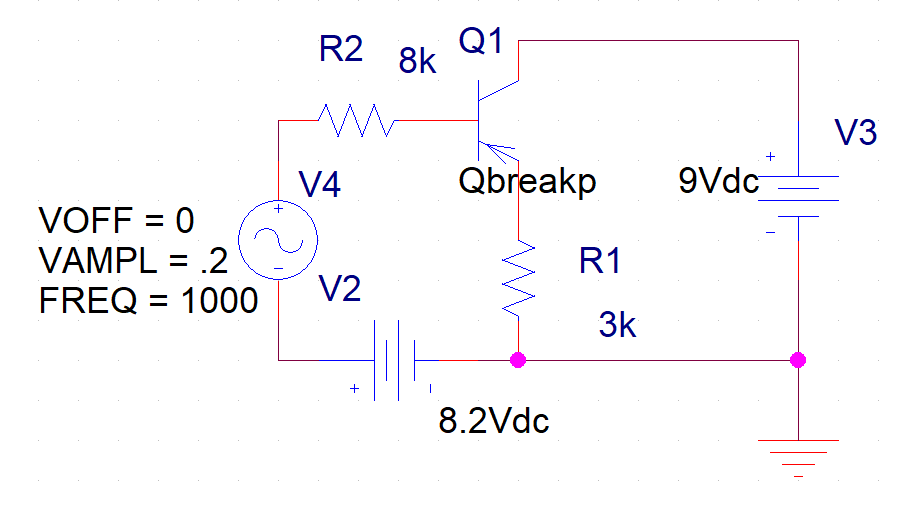
\includegraphics[width=.9\textwidth]{Figures/HW6-2a}
              \caption{PSPICE Circuit Construction}
              \label{fig:1}
            \end{figure}

          \item Running the bias point simulation, we obtain:

            \begin{figure}[H]
              \centering
              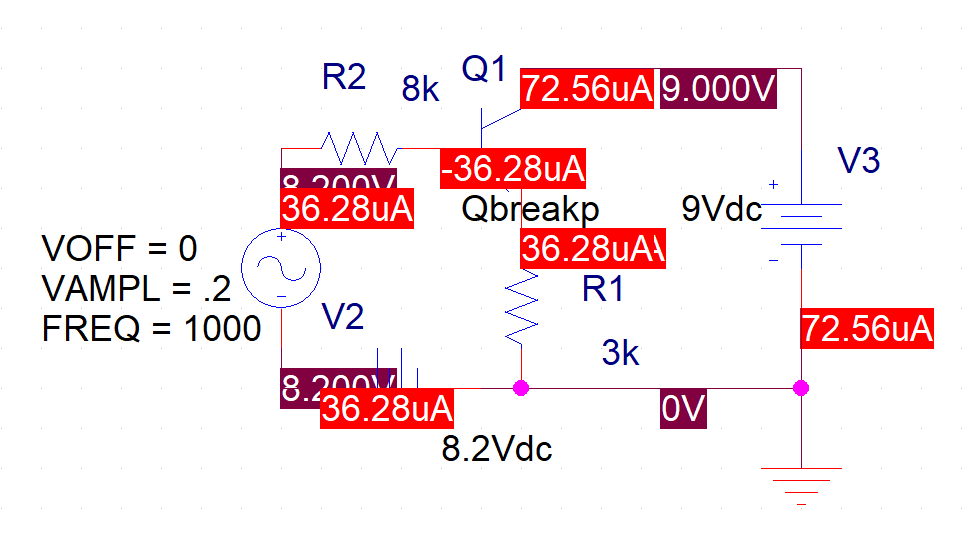
\includegraphics[width=.9\textwidth]{Figures/HW6-2b}
              \caption{Bias Point Simulation Results}
              \label{fig:2}
            \end{figure}

          \item First, we find the ``hard set'' value of $\beta$, highlighted below:

            \begin{figure}[H]
              \centering
              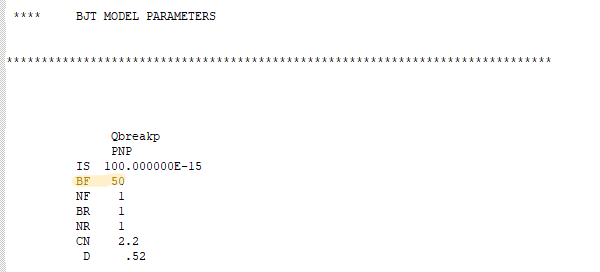
\includegraphics[width=.9\textwidth]{Figures/HW6-2c}
              \caption{Device $\beta$ Value}
              \label{fig:3}
            \end{figure}

            We may then see the values of $\beta_{DC}$ and $\beta_{AC}$:

            \begin{figure}[H]
              \centering
              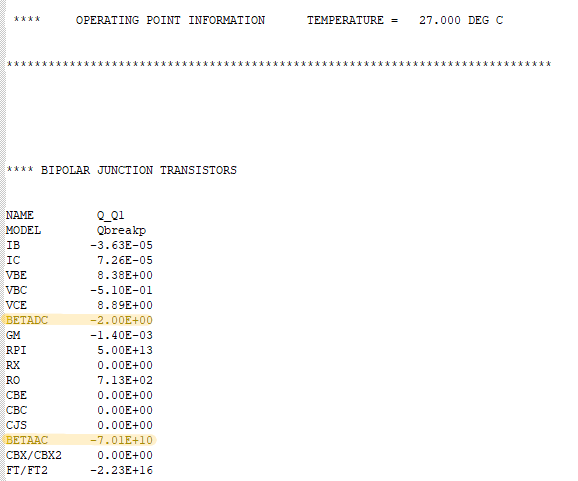
\includegraphics[width=.9\textwidth]{Figures/HW6-2d}
              \caption{Operating Point Simulation Values}
              \label{fig:4}
            \end{figure}

          \item 

            Simulating produced the following transients:

            \begin{figure}[H]
              \centering
              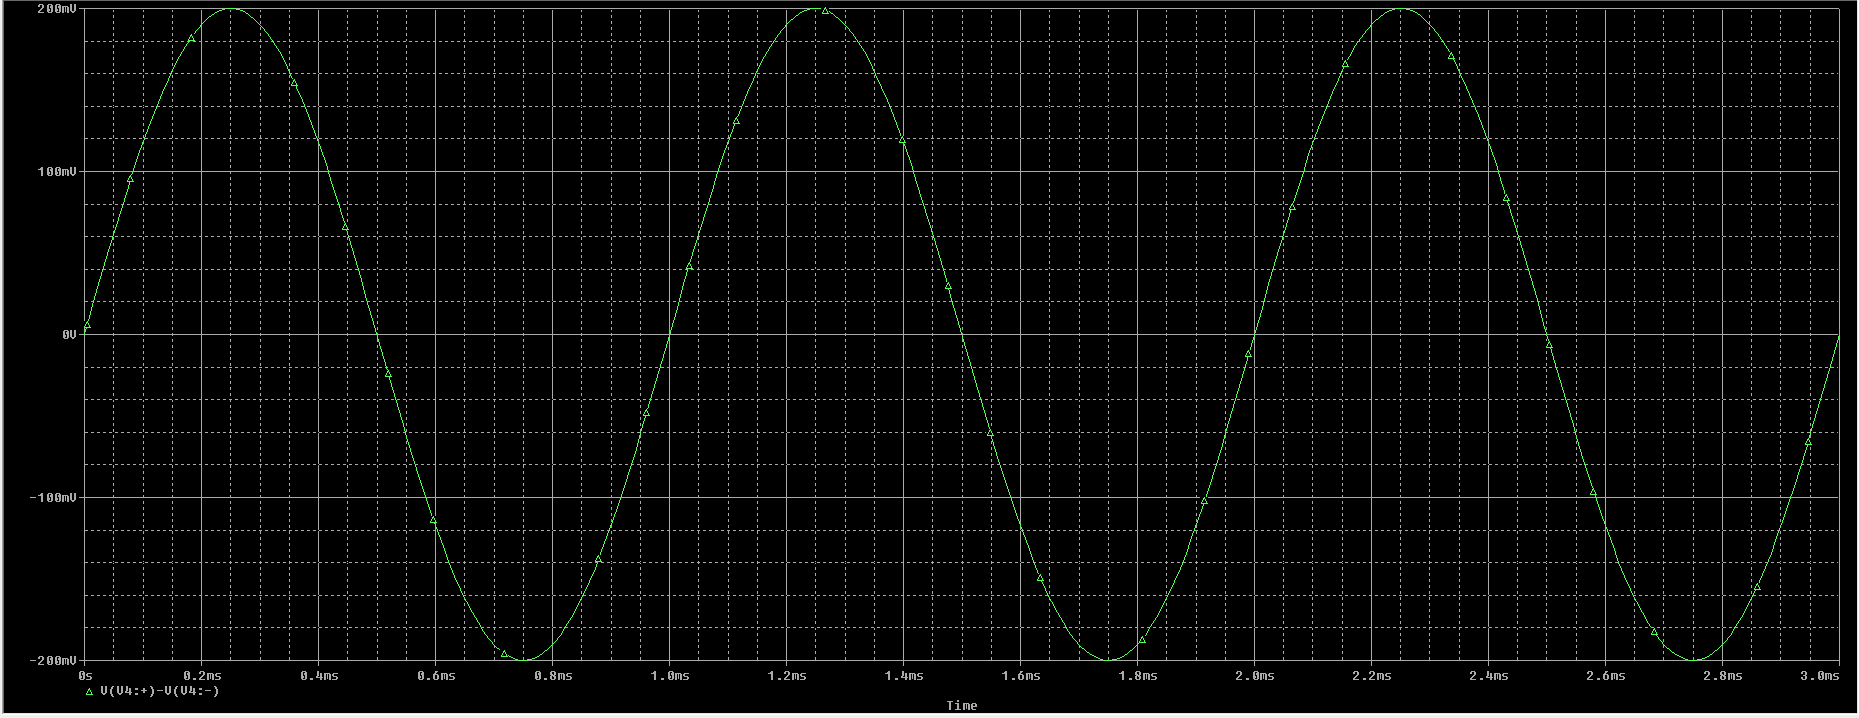
\includegraphics[width=.9\textwidth]{Figures/HW6-2e}
              \caption{Circuit $V_{in}(t)$ Value}
              \label{fig:5}
            \end{figure}

            \begin{figure}[H]
              \centering
              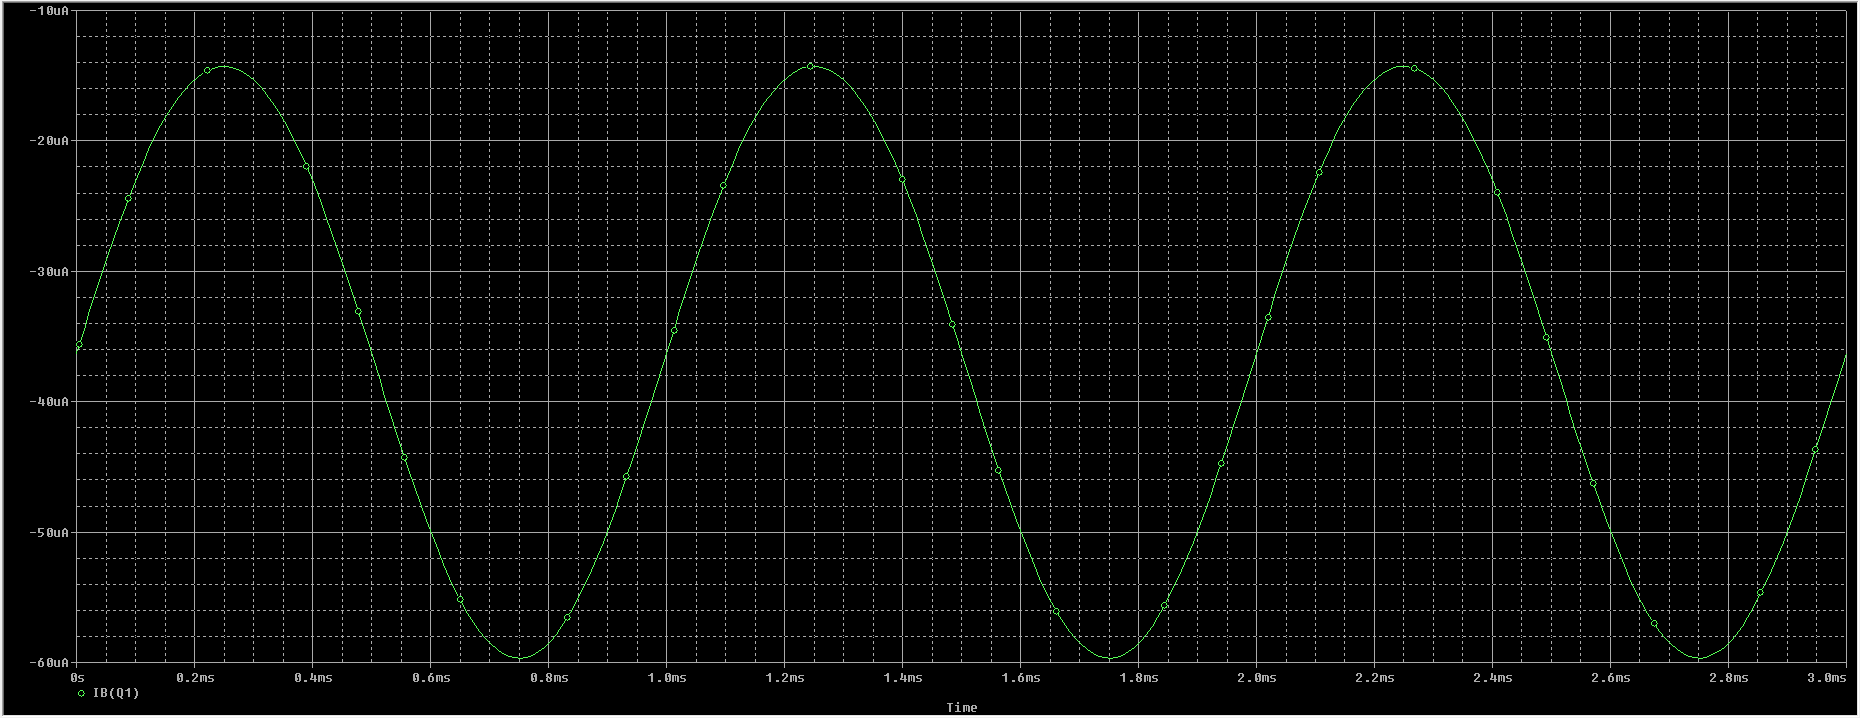
\includegraphics[width=.9\textwidth]{Figures/HW6-2f}
              \caption{Circuit $I_B(t)$ Value}
              \label{fig:6}
            \end{figure}

            \begin{figure}[H]
              \centering
              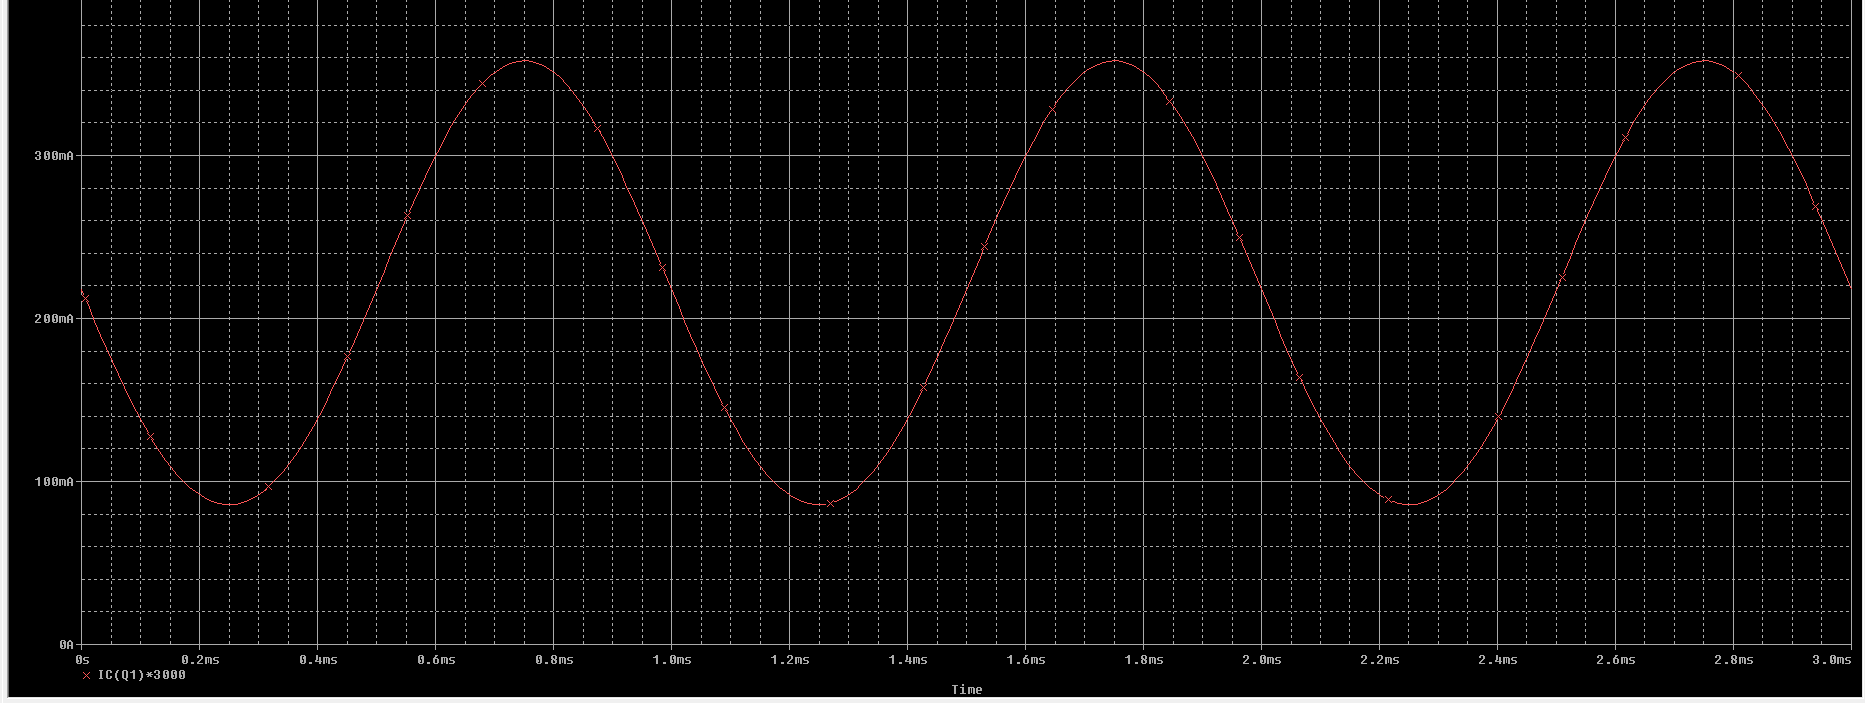
\includegraphics[width=.9\textwidth]{Figures/HW6-2g}
              \caption{Circuit $V_o(t)$ Value}
              \label{fig:7}
            \end{figure}

            We may see that the simulated circuit, more or less, follows the expected values calculated in part (a).

        \end{enumerate}

    \end{enumerate}

  \item

    \begin{enumerate}

      \item 

        We use KVL at the base-emitter loop to obtain:

        $$12=(I_C+I_B)R_C+R_1I_B+.7+R_EI_E$$

        And at the collector-emitter loop, we get:

        $$12=(I_C+I_B)R_C+V_{CE}+R_EI_E$$

        We may apply:

        $$I_E=(\beta+1)I_B\quad\text{ and }\quad I_E=I_B+I_C$$

        To get:

        $$12=(I_E)R_C+R_B\left( \frac{I_E}{\beta+1} \right)+.7+R_EI_E$$

        Substituting known values, we get:

        $$11.3=(I_E)1000+10000\left( \frac{I_E}{\beta+1} \right)+200I_E$$

        Solving for $I_E$, we get:

        $$1396.1I_E=11.3$$
        $$\boxed{I_E=8.0941[\si{\milli\ampere}]\Big|_{\beta=50}}$$

        From this, we get:

        $$I_B=\frac{I_E}{\beta+1}\quad\text{ and }\quad I_C=\left( \frac{\beta}{\beta+1} \right)I_E$$
        $$\boxed{I_B=158.71[\si{\micro\ampere}]\quad\text{ and }\quad I_C=7.9354[\si{\milli\ampere}]\Big|_{\beta=50}}$$

        Using our collector-emitter loop, we see:

        $$V_{CE}=12-I_E(R_C+R_E)$$
        $$V_{CE}=12-8.0941(.2+1)$$
        $$\boxed{V_{CE}=2.2871[\si{\volt}]\Big|_{\beta=50}}$$

        For $\beta=250$, we repeat the analysis at this point:

        $$11.3=(I_E)1000+10000\left( \frac{I_E}{\beta+1} \right)+200I_E$$

        This gives us:

        $$1239.8I_E=11.3$$
        $$\boxed{I_E=9.1141[\si{\milli\ampere}]\Big|_{\beta=250}}$$

        Then:

        $$\boxed{I_B=36.311[\si{\micro\ampere}]\quad\text{ and }\quad I_C=9.0778[\si{\milli\ampere}]\Big|_{\beta=250}}$$

        Finally, we get:

        $$V_{CE}=12-9.1141(1.2)$$
        $$\boxed{V_{CE}=1.0631[\si{\volt}]}$$

      \item Repeating Part (a) with $R_E=0$, we get:

        $$11.3=(I_E)1000+10000\left( \frac{I_E}{\beta+1} \right)$$

        From which we obtain:

        $$1039.8I_E=11.3\quad\text{ and }\quad1196.1I_E=11.3$$
        $$\boxed{I_E=.010867[\si{\ampere}]\Big|_{\beta=250}\quad\text{ and }\quad I_E=9.4474[\si{\milli\ampere}]\Big|_{\beta=50}}$$

        From this, we can get:

        $$\boxed{I_B=43.295[\si{\micro\ampere}]\quad\text{ and }\quad I_C=.010824[\si{\ampere}]\Big|_{\beta=50}}$$
        $$\boxed{I_B=185.24[\si{\micro\ampere}]\quad\text{ and }\quad I_C=9.2622[\si{\milli\ampere}]\Big|_{\beta=250}}$$

        Finally, we reach:

        $$V_{CE}=12-I_E(1000)$$
        $$V_{CE}=12-10.867\quad\text{ and }\quad 12-9.4474$$
        $$\boxed{V_{CE}=1.133[\si{\volt}]\Big|_{\beta=250}\quad\text{ and }\quad V_{CE}=2.5526[\si{\volt}]\Big|_{\beta=50}}$$

      \item The circuit was constructed as follows:

        \begin{figure}[H]
          \centering
          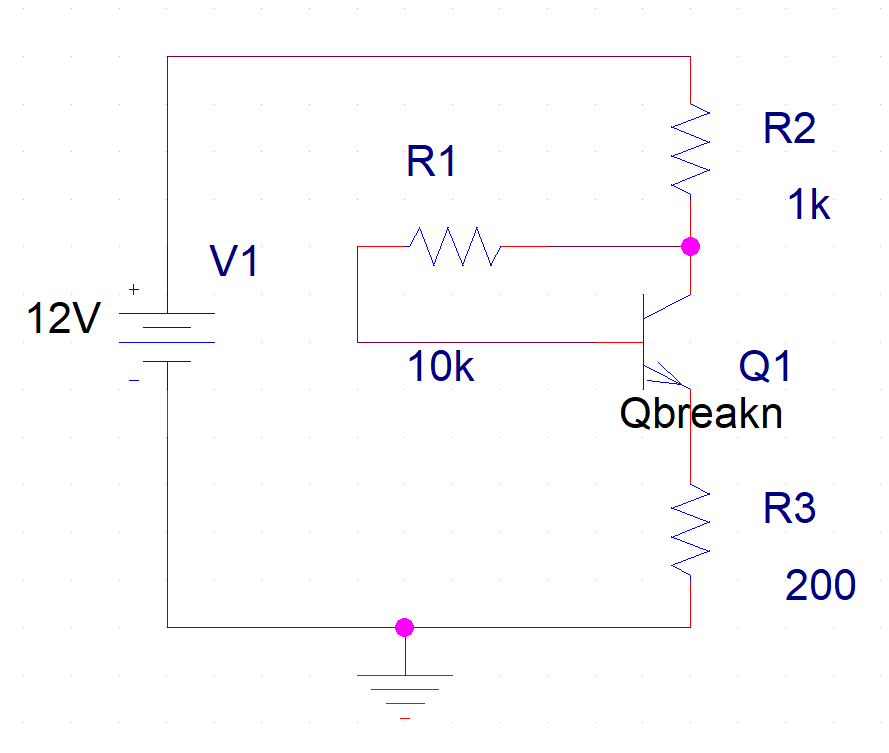
\includegraphics[width=.9\textwidth]{Figures/HW6-3a}
          \caption{Circuit Construction}
          \label{fig:8}
        \end{figure}

        We then simulate with $\beta=50$:

        \begin{figure}[H]
          \centering
          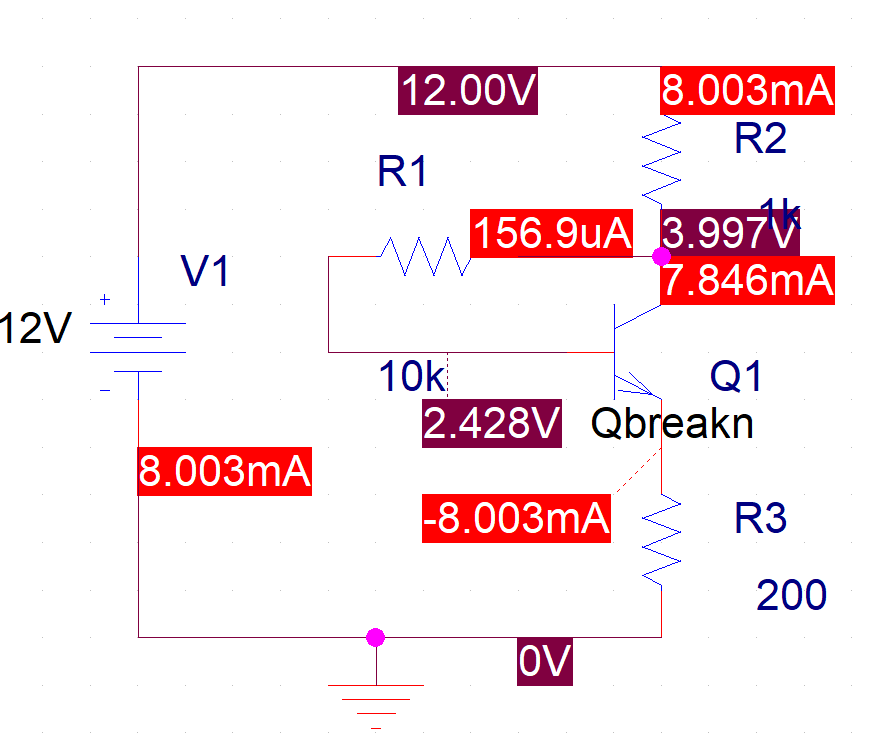
\includegraphics[width=.9\textwidth]{Figures/HW6-3b}
          \caption{$\beta=50$ Simulation Result}
          \label{fig:9}
        \end{figure}

        And then with $\beta=250$:

        \begin{figure}[H]
          \centering
          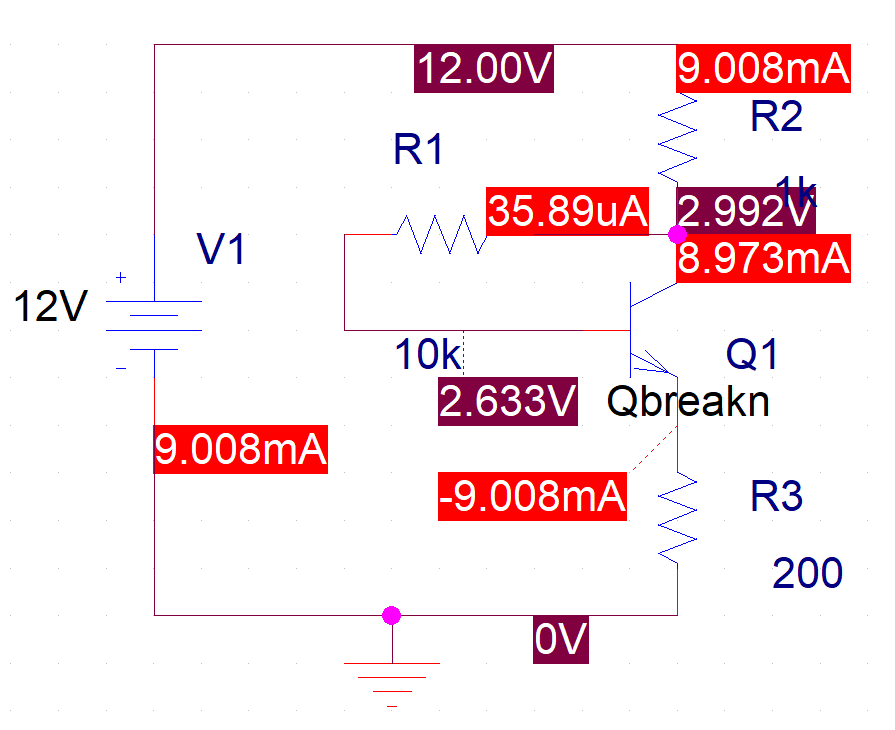
\includegraphics[width=.9\textwidth]{Figures/HW6-3c}
          \caption{$\beta=250$ Simulation Result}
          \label{fig:10}
        \end{figure}

        We may observe that the simulation result is quite similar to what we calculated in Part (a), with the biggest difference being a slightly offset $V_{CE}$ value.

    \end{enumerate}

\end{enumerate}

\end{document}

